\documentclass[a4paper,12pt]{article}
\usepackage[utf8]{inputenc}
\usepackage{longtable}
\usepackage{geometry}
\usepackage{hyperref}
\usepackage{array}
\usepackage{caption}
\usepackage{booktabs}
\geometry{margin=1in}
\usepackage{graphicx}
\usepackage{float}
\usepackage{hyperref}
\title{Research For Taxi Tap\\Taxi Tap by Git It Done}
\date{}
\begin{document}
\maketitle
\begin{figure}[H]
  \centering
  
\includegraphics[width=0.5\textwidth]{LogoGroup.png} 
\end{figure}
\begin{figure}[H]
  \centering
  
\includegraphics[width=0.5\textwidth]{LogoTaxiTap.png} 
\end{figure}
\newpage
\tableofcontents
\newpage
\section{Introduction}
During the course of this project, Taxi Tap, we had to do quite a bit of research to ensure that we have an application that is well thought out and takes both passengers and drivers into consideration. In the following, we discuss the sections of research we had to do to enhance our system and ensure that users are satisfied.

\section{Payment System}
As you will see when using the application, we do not have a digital payment system integrated into our mobile application. This is because after doing user research we came to the conclusion that a digital payment system is not ideal for the taxi system we have today.\newline

After speaking to multiple individuals who are taxi passengers, we understood that the passengers, as well as the drivers, are comfortable with the cash payment system. Thus for our system we decided to use this information to our advantage.\newline

Since there is already an established trust between passengers and drivers, we decided to enhance our application by integrating some sort of cash payment system. This payment system focuses on helping the passenger (the one who sits at the front), to easily make sure everyone gets enough change and that all passengers have paid the correct amount. The driver can also see payments that are in the waiting state and passengers that have not paid to ensure that drivers get the most out of our application.

\section{South African Taxi Industry Context}
The South African minibus taxi industry operates under a unique regulatory and operational framework that significantly influenced the design of Taxi Tap. Understanding this context was crucial for developing a system that works with, rather than against, the established industry structure.

\subsection{Route Registration and Ownership}
In South Africa, taxi routes are formally registered with taxi associations, which act as governing bodies for specific geographic areas and route networks. Multiple associations can operate similar or overlapping routes, creating a complex network of transportation options. Drivers typically pay membership fees to join these associations, which in turn assign them to specific routes. This assignment is relatively fixed, drivers cannot deviate from their registered routes to accommodate individual passenger requests, a constraint that fundamentally shaped our approach to journey planning.

The ownership model also varies: drivers may own their vehicles or operate association-owned taxis. Owner-drivers typically earn higher profits but bear the full cost of vehicle maintenance and operation. This economic reality reinforces the importance of route efficiency and passenger volume, factors we considered when designing features like the split payment system.

\subsection{Operational Constraints}
Unlike ride-hailing services where drivers can navigate freely to any destination, taxi drivers in South Africa must adhere strictly to their assigned routes. This constraint means passengers cannot simply request door-to-door service to arbitrary locations. Instead, passengers must understand the route network and plan journeys that align with available routes. This created the primary problem our application addresses: how can passengers efficiently navigate a complex network of fixed routes to reach their destinations?

Our research into these operational realities led to two key features: comprehensive route mapping with accurate stop information, and intelligent multi-leg journey planning for destinations not directly reachable by a single route.

\section{Taxi Route Mapping Research}
Accurate route information forms the foundation of Taxi Tap's journey planning capabilities. Without reliable data on where taxis travel and where they stop, passengers cannot effectively plan their journeys. This section details our systematic approach to acquiring, processing, and validating taxi route data.

\subsection{Data Acquisition}
Route data was sourced from official government documents containing route registrations submitted by taxi associations. These PDF documents contained approximately 100 registered routes across various associations operating in the target service area. The documents represented the formal, legally registered routes that drivers are authorized to operate.

While these official documents provided legitimate route information, they presented significant challenges. The directions were written in natural language, often mixing formal addresses with colloquial place names familiar to locals but not standardized in mapping databases. Additionally, the format varied considerably between different associations' submissions, with no standardized template or structure.

\subsection{Data Cleaning and Transformation Process}
The transformation of raw PDF documents into structured, geocoded route data required a comprehensive data science pipeline implemented in Python. This process exemplified the full data analysis lifecycle: data acquisition, cleaning, transformation, enrichment, and validation.

\subsubsection{PDF Parsing and Text Extraction}
The initial challenge involved extracting usable text from PDF documents with varying formats. Using Python's text extraction libraries, we developed a parser that could handle the inconsistent document structures. The primary libraries employed included:

\begin{itemize}
\item \texttt{re} for regular expression pattern matching to identify route structures
\item \texttt{requests} for API calls to geocoding services
\item \texttt{json} for structured data serialization
\item Standard Python logging for monitoring the extraction process
\end{itemize}

The parser identified route names, stop sequences, and directional information from the unstructured text. This required developing pattern recognition rules that could adapt to format variations while maintaining accuracy.

\subsubsection{Address Normalization}
Once text was extracted, the next challenge was normalizing the diverse address formats. Directions included:
\begin{itemize}
\item Official street addresses
\item Colloquial place names used by locals
\item Landmark references
\item Informal location descriptions
\end{itemize}

We implemented conditional logic to handle common variations, such as different spellings of the same location or multiple names for the same landmark. Fortunately, many informal locations had been added to mapping databases by South African contributors, albeit as unofficial listings. This community-contributed geographic data proved invaluable for resolving ambiguous location references.

\subsection{Reverse Geocoding Implementation}
Converting textual location descriptions into precise latitude and longitude coordinates required robust geocoding. We implemented a two-tier approach:

\begin{enumerate}
\item \textbf{Primary Service:} OpenStreetMap's Nominatim API served as our primary geocoding service due to its comprehensive coverage of South African locations and generous usage limits.
\item \textbf{Fallback Service:} For locations that failed with OpenStreetMap, we implemented fallback queries to Google Maps Geocoding API, using the limited free tier strategically for difficult cases.
\end{enumerate}

This dual-service approach achieved a geocoding success rate exceeding 90 percent. For the remaining cases where automated geocoding failed, manual intervention was employed. When a stop name could not be resolved to coordinates, we used the coordinates of the stop itself as a reference point and retained the original stop name for passenger recognition.

The geocoding script incorporated rate limiting and error handling to manage API quotas and ensure robust operation:

\begin{verbatim}
import time
import requests
from typing import Optional, Tuple

def geocode_location(location: str) -> Optional[Tuple[float, float]]:
    # Primary: OpenStreetMap
    # Fallback: Google Maps
    # Rate limiting and retry logic
\end{verbatim}

\subsection{Data Storage and Structure}
Successfully geocoded routes were initially stored as JSON files, providing a human-readable intermediate format that facilitated debugging and validation. Each route object contained:
\begin{itemize}
\item Route identifier and name
\item Associated taxi association
\item Ordered list of stops with coordinates
\item Metadata such as estimated duration and base fare
\end{itemize}

This structured data was subsequently migrated to our backend database, where it powers real-time route queries and journey planning algorithms in the production application.

\subsection{Validation and Quality Assurance}
A limitation of our approach was the absence of systematic validation against ground truth. We operated under the assumption that government-submitted route registrations were accurate, as these represent the legal routes associations are authorized to operate. While this pragmatic approach allowed rapid development, it represents an area for future improvement through field validation or crowdsourced verification.

\section{Multi-Leg Journey Planning Research}
Many destination pairs in the taxi network cannot be connected by a single route. Passengers must transfer between routes operated by different associations, often requiring walking between stops. This section describes our research into algorithmic journey planning across multiple taxi routes.

\subsection{Problem Definition}
The multi-leg journey problem can be formally stated: Given an origin point O and destination point D, find a sequence of taxi rides and walking transfers that connects O to D, where each taxi ride must follow a registered route and walking distances must be reasonable.

This differs from traditional route planning in several ways:
\begin{itemize}
\item Routes are fixed and cannot deviate
\item Transfers must occur at or near route stops
\item Multiple associations operate independently
\item Walking between stops must be factually reasonable for passengers
\end{itemize}

\subsection{Intersection Detection Algorithm}
The foundation of multi-leg planning is identifying where different routes intersect or come sufficiently close to enable transfers. We developed a Python-based algorithm using geospatial analysis libraries:

\begin{verbatim}
import pandas as pd
import networkx as nx
from typing import List, Dict, Tuple, Set
import math
\end{verbatim}

The algorithm computes distances between all stops across different routes using the Haversine formula, which calculates great-circle distances between coordinate pairs on a sphere. For each pair of stops from different routes, if the distance falls below a threshold of 3 kilometers, the stops are marked as potential transfer points.

This threshold was chosen to represent a reasonable walking distance for passengers: approximately 30 to 45 minutes of walking at average pace. While longer than ideal, it reflects the reality of sparse route coverage in some areas and the necessity of transfers for reaching certain destinations.

\subsection{Transfer Point Eligibility}
Not all intersections make viable transfer points. Our algorithm evaluates several criteria:

\begin{itemize}
\item \textbf{Distance:} Stops must be within 3 kilometers
\item \textbf{Route Direction:} The sequence must make logical sense (origin route progresses toward the transfer point, destination route progresses from transfer point toward destination)
\item \textbf{Association Diversity:} Transfers should connect routes from different associations, as same-association routes typically offer direct connections
\end{itemize}

The algorithm constructs a transfer graph where nodes represent route stops and edges represent valid transfers, weighted by walking distance and estimated time.

\subsection{Journey Construction}
Given origin and destination coordinates, the multi-leg planner:

\begin{enumerate}
\item Identifies routes with stops near the origin (within 1 kilometer walking distance)
\item Identifies routes with stops near the destination (within 1 kilometer)
\item Searches the transfer graph for paths connecting origin-accessible routes to destination-accessible routes
\item Validates that stop sequences respect route order (no backtracking)
\item Calculates total cost and estimated time for each viable journey
\item Returns the top options ranked by total cost
\end{enumerate}

Currently, the system supports journeys with up to two legs (one transfer), balancing complexity with usability. Future enhancements could extend this to three-leg journeys for more comprehensive coverage.

\subsection{Implementation Evolution}
The multi-leg planning system was first prototyped in Python using libraries such as \texttt{pandas} for data manipulation, \texttt{networkx} for graph algorithms, and \texttt{folium} for visualization. This prototype validated the approach and allowed experimentation with different distance thresholds and ranking criteria.

The production implementation was then developed in TypeScript for integration with our backend infrastructure. The TypeScript version implements the same algorithmic logic while interfacing with our real-time database and providing low-latency responses to mobile clients. Key components include:

\begin{itemize}
\item Distance calculation using the Haversine formula
\item Dynamic fare calculation based on distance traveled
\item Route filtering by driver availability
\item Transfer point detection with configurable distance thresholds
\item Journey validation ensuring proper stop sequencing
\end{itemize}

\subsection{Visualization and Verification}
To verify the correctness of our intersection detection and journey planning, we created visualizations using Python's \texttt{folium} library, which generates interactive maps. These visualizations served multiple purposes:

\begin{itemize}
\item Verifying that detected intersections were geometrically correct
\item Identifying potential issues with route data quality
\item Demonstrating multi-leg journey options to stakeholders
\item Providing a reference for future system enhancements
\end{itemize}

Figure \ref{fig:route_stops} shows the mapped route network with all stops visualized, demonstrating the comprehensive coverage achieved through our data processing pipeline. Figure \ref{fig:transfer_points} highlights detected transfer points between routes, showing where passengers can switch between different taxi services. Figure \ref{fig:complete_network} presents the complete network view with both stops and transfer points, illustrating the full complexity of the multi-leg journey planning problem.

\begin{figure}[H]
  \centering
  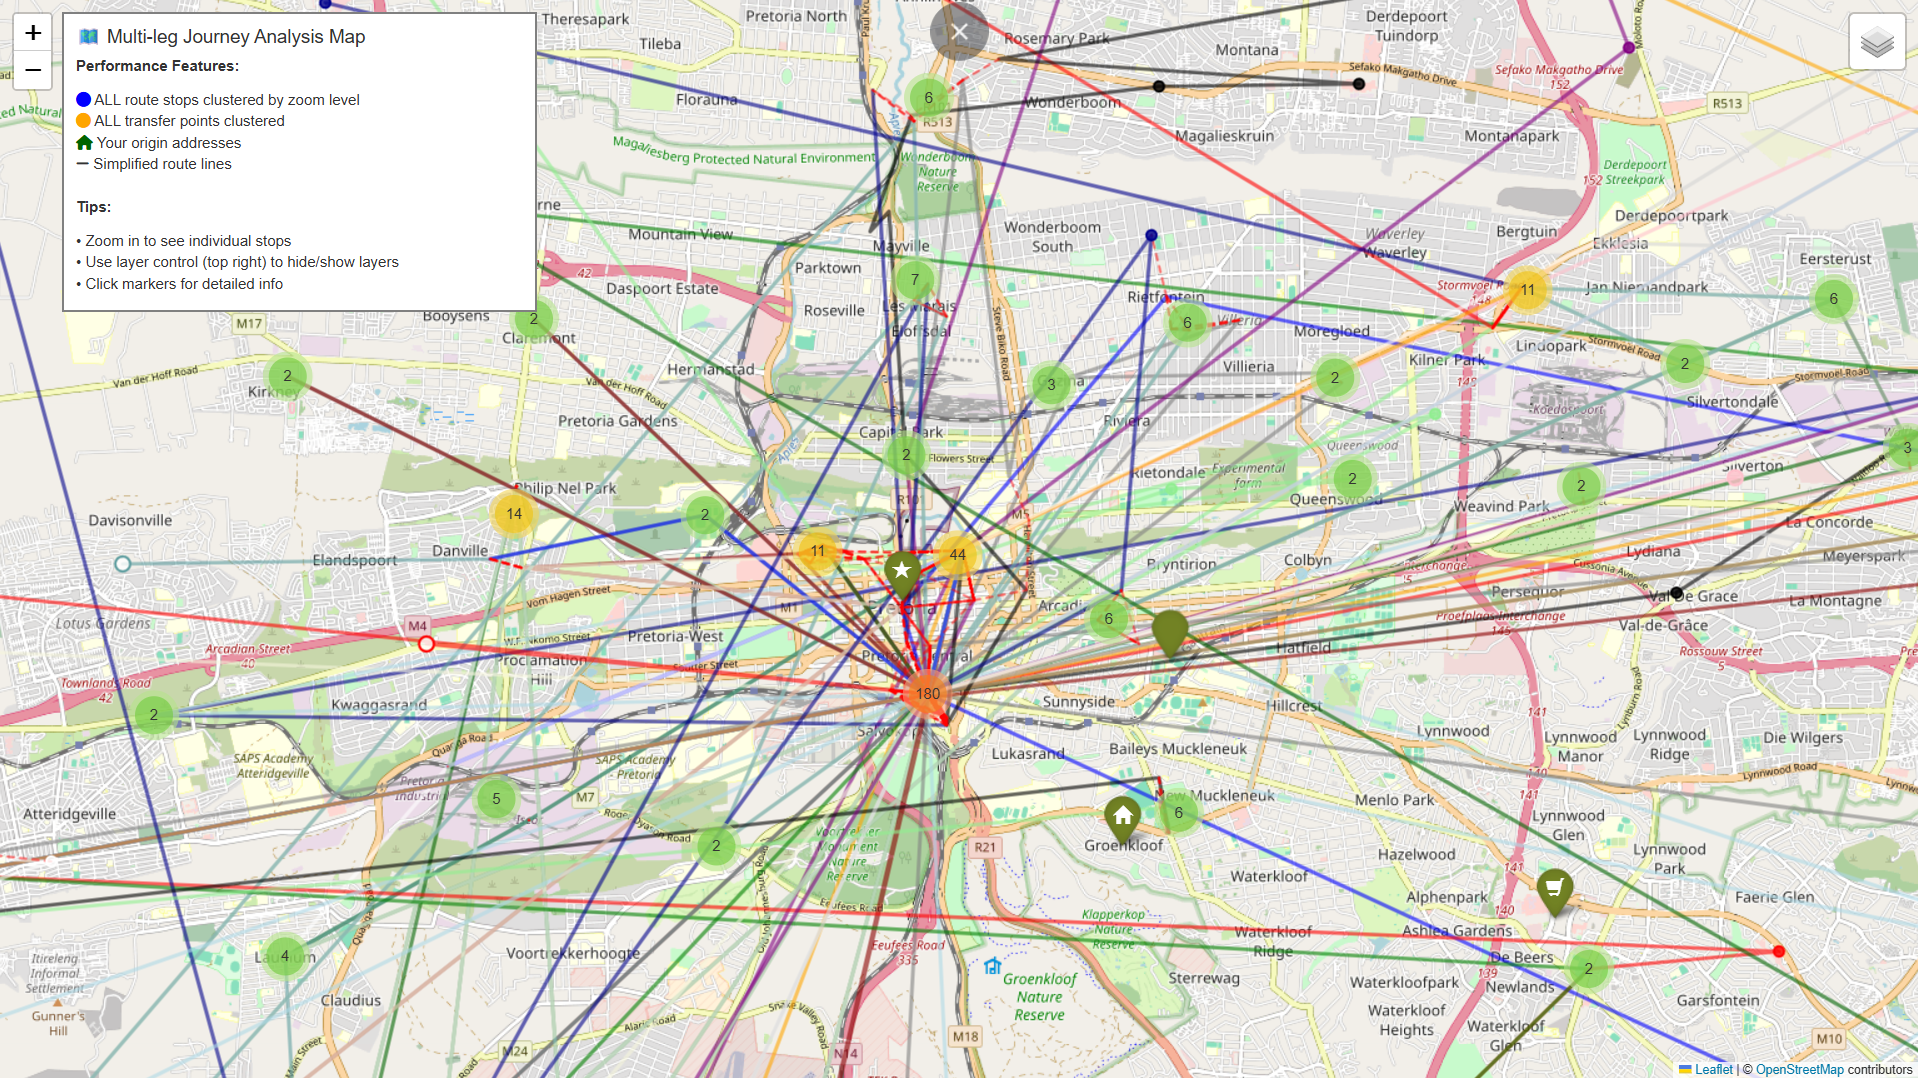
\includegraphics[width=0.8\textwidth]{route_stops_map.png}
  \caption{Mapped taxi routes showing all geocoded stops across the service area}
  \label{fig:route_stops}
\end{figure}

\begin{figure}[H]
  \centering
  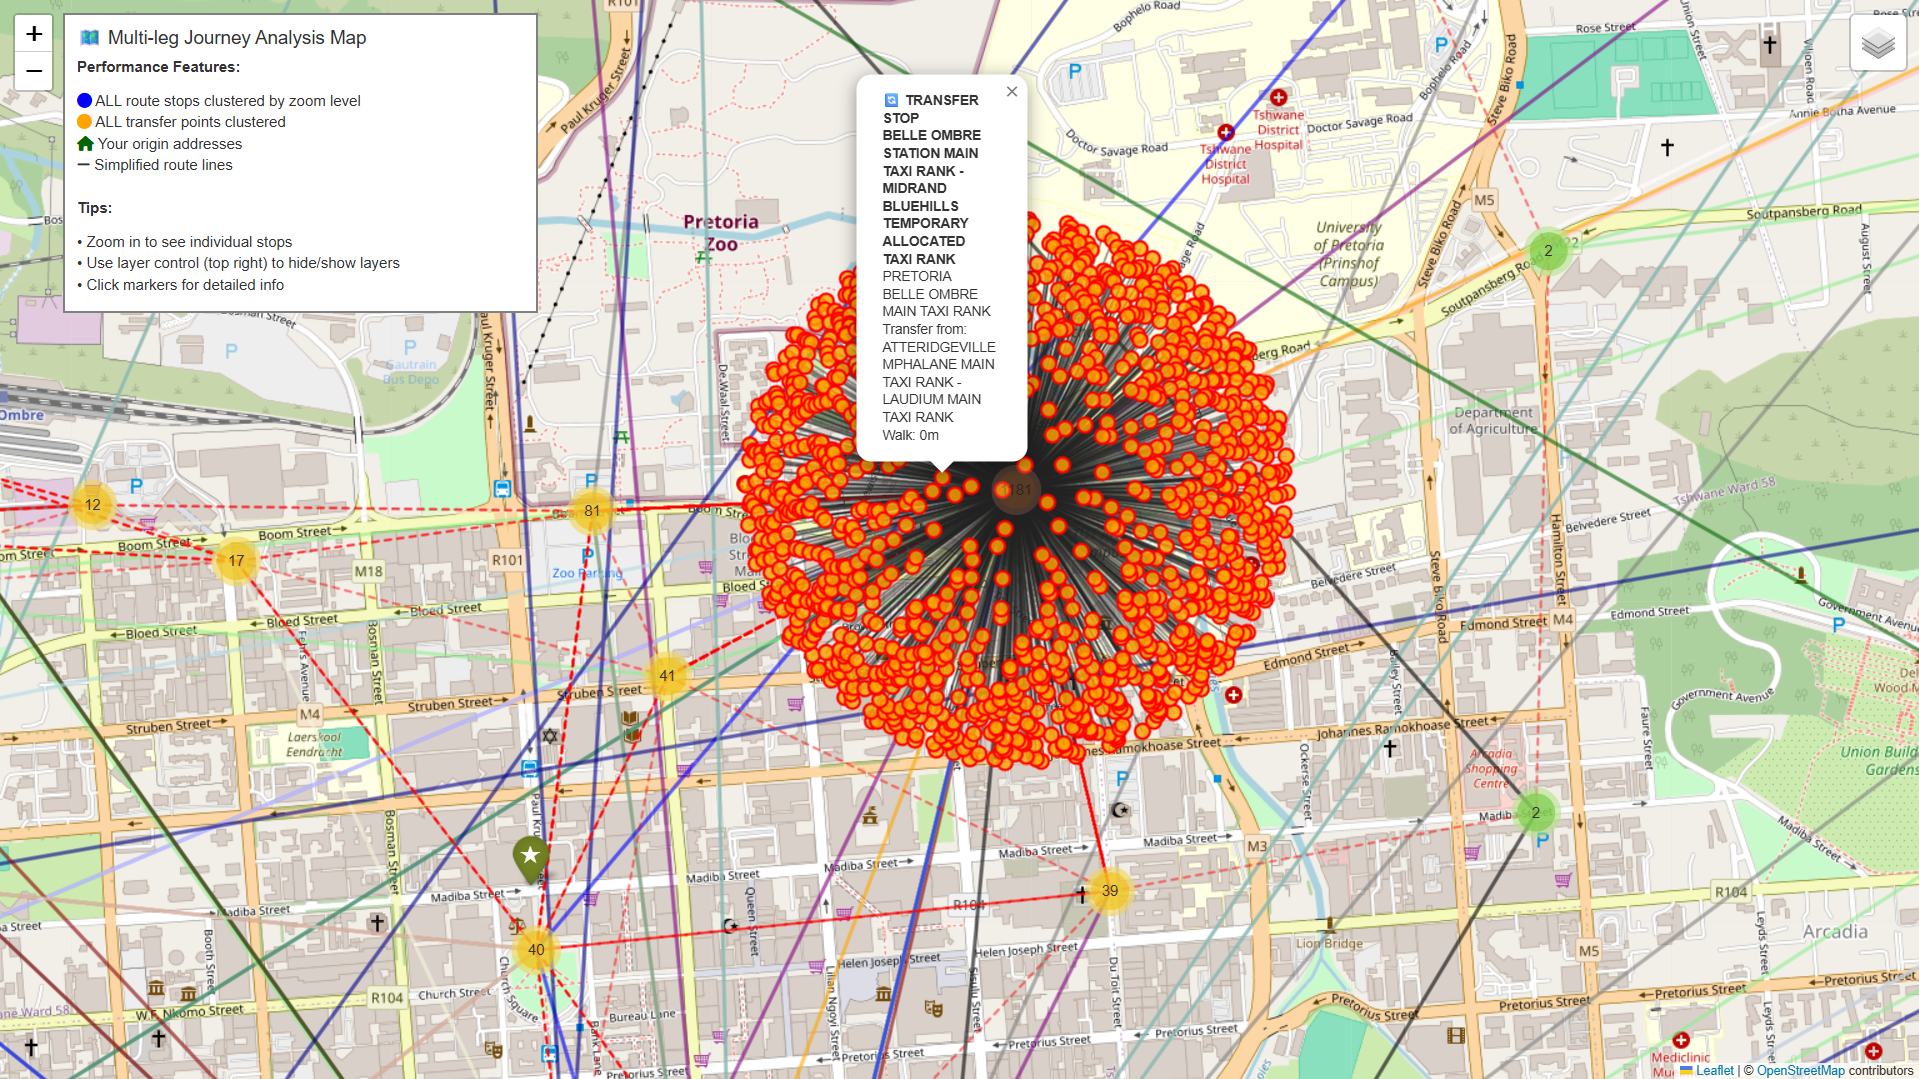
\includegraphics[width=0.8\textwidth]{transfer_points_map.png}
  \caption{Detected transfer points where passengers can switch between routes}
  \label{fig:transfer_points}
\end{figure}

\begin{figure}[H]
  \centering
  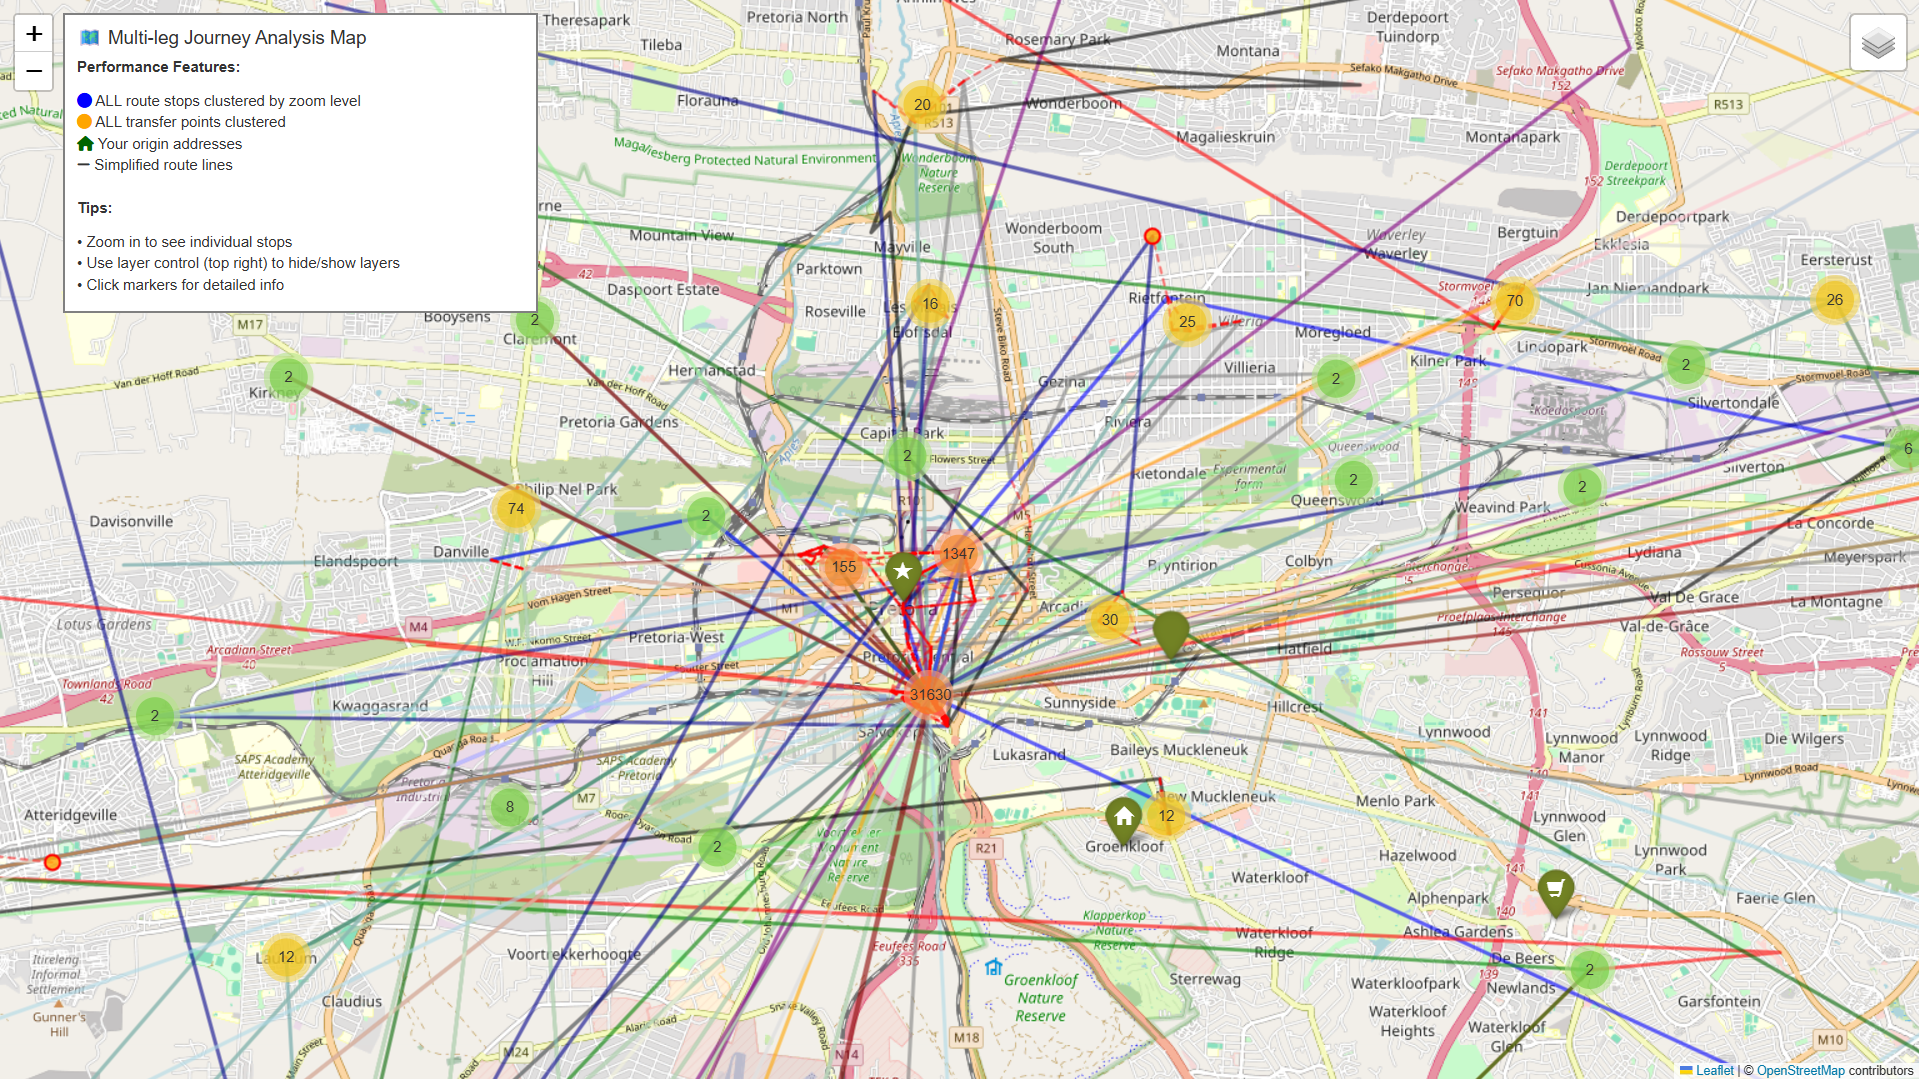
\includegraphics[width=0.8\textwidth]{complete_network_map.png}
  \caption{Complete network view showing routes, stops, and transfer points}
  \label{fig:complete_network}
\end{figure}

\section{Technical Challenges and Solutions}
Throughout the research and development process, several significant challenges emerged that required innovative solutions.

\subsection{PDF Parsing Complexity}
The primary technical challenge was extracting structured information from inconsistently formatted PDF documents. Different taxi associations submitted route information using varying templates, naming conventions, and organizational structures. Our solution involved developing flexible parsing rules that could identify key elements (route names, stop sequences, directional indicators) regardless of document structure, while logging ambiguous cases for manual review.

\subsection{Geocoding Accuracy}
Achieving high geocoding accuracy for colloquial and informal location names proved difficult. Many stops are known locally by names that do not appear in official mapping databases. Our multi-service approach with OpenStreetMap and Google Maps fallback significantly improved success rates. Additionally, leveraging community-contributed geographic data in OpenStreetMap proved invaluable for resolving South African-specific location references.

The remaining geocoding failures (less than 10 percent of stops) were handled gracefully by using stop coordinates as positional anchors while preserving human-readable names for passenger recognition.

\subsection{Performance Optimization}
Computing all possible multi-leg journeys across 100 routes with thousands of stops created performance concerns. The transfer points are calculated dynamically in the application code using the Haversine distance formula between stops from different routes. To optimize this, routes are first filtered by driver availability in the journey area before computing transfer points, significantly reducing the number of calculations required. 

\section{Research Impact on Application Design}
The research detailed in this document directly shaped Taxi Tap's core functionality and user experience.

\subsection{Route-Centric User Interface}
Understanding that routes are fixed and drivers cannot deviate informed our decision to present route information prominently in the user interface. Rather than hiding route complexity, we embrace it, showing passengers which routes serve their journey and where they need to board and alight.

\subsection{Transfer Guidance}
The multi-leg journey planner translates complex network analysis into simple, actionable guidance for passengers. Users receive step-by-step instructions: which route to take first, where to transfer, how far to walk, which route to take next, and the total estimated cost. This transforms the cognitive burden of network planning from the passenger to the application.

\subsection{Cash Payment Integration}
As discussed in Section 2, our research into payment preferences revealed strong attachment to cash transactions. This finding, combined with our route and journey planning research, led to a holistic design that respects existing industry practices while providing modern conveniences.

\subsection{Scalability Considerations}
The data processing pipeline is designed for scalability. As additional routes are registered or existing routes are modified, the Python scripts can be re-run to update the route database and transfer point graph. This ensures Taxi Tap can grow alongside the evolving taxi industry without requiring architectural changes.

\section{Future Research Directions}
While our current research provides a solid foundation for Taxi Tap, several areas warrant future investigation:

\begin{itemize}
\item \textbf{Ground Truth Validation:} Systematic validation of route data through field studies or driver surveys
\item \textbf{Real-Time Route Updates:} Integration with taxi association systems to receive automatic route updates
\item \textbf{Three-Leg Journeys:} Extending multi-leg planning to support additional transfers for more comprehensive coverage
\item \textbf{Dynamic Transfer Points:} Incorporating real-time traffic and safety data to recommend optimal transfer locations
\item \textbf{Crowdsourced Corrections:} Enabling drivers and passengers to suggest route corrections or additional stops
\item \textbf{Predictive Analytics:} Using historical journey data to estimate wait times and optimal departure times
\end{itemize}

\section{Conclusion}
The research undertaken for Taxi Tap demonstrates the value of understanding domain context before implementing technical solutions. By thoroughly investigating the South African taxi industry's unique operational model, we developed a system that works within existing constraints rather than fighting against them. The data science pipeline for route mapping and the algorithmic approach to multi-leg journey planning represent significant technical contributions that make taxi travel more accessible and understandable for passengers while respecting the established industry structure.

\end{document}